\section{Work plan — Work packages, deliverables}

Brief description of the section

\subsection{Overall Structure}
%Brief presentation of the overall structure of the work plan. \textbf{Network diagram SOLO de los WP o diagrama explicativo del proyecto. El network diagram que tenemos ahora está en D2 Apartado 3.2.}

The DEOS-UD project is composed by 7 different work packages which are interrelated as shown in Figure \ref{overallstructure}. WP1 deals with project management and will ensure the proper coordination of project activities and the achievement of project objectives. WP2 is related to the quality and the administration of the project in terms of human resources, documentation management and quality, periodic monitoring and will also stablish the financial plan of the project. WP3 will study the current baseline designs for the studied technologies (payload, modular system and urban development application) in the sector and will establish the potential areas of improvement and the requirements needed to achieve the new technologies proposed. WP4 is in charge of design the output products of the project. This WP has a strong relationship with WP5 which is in charge of manufacture the prototype and validate it. Good intercommunication between these WPs is needed in order to obtain a final product that achieves the requirements imposed by WP3. WP6 aims to create a methodology to enable the future use of the new technologies developed during the project, assuring the continuity of them. And last but not least, WP7 will ensure the project results are communicated and disseminated to the appropriate audiences, establishing new knowledge into the society.

\begin{figure}[H]
\centering
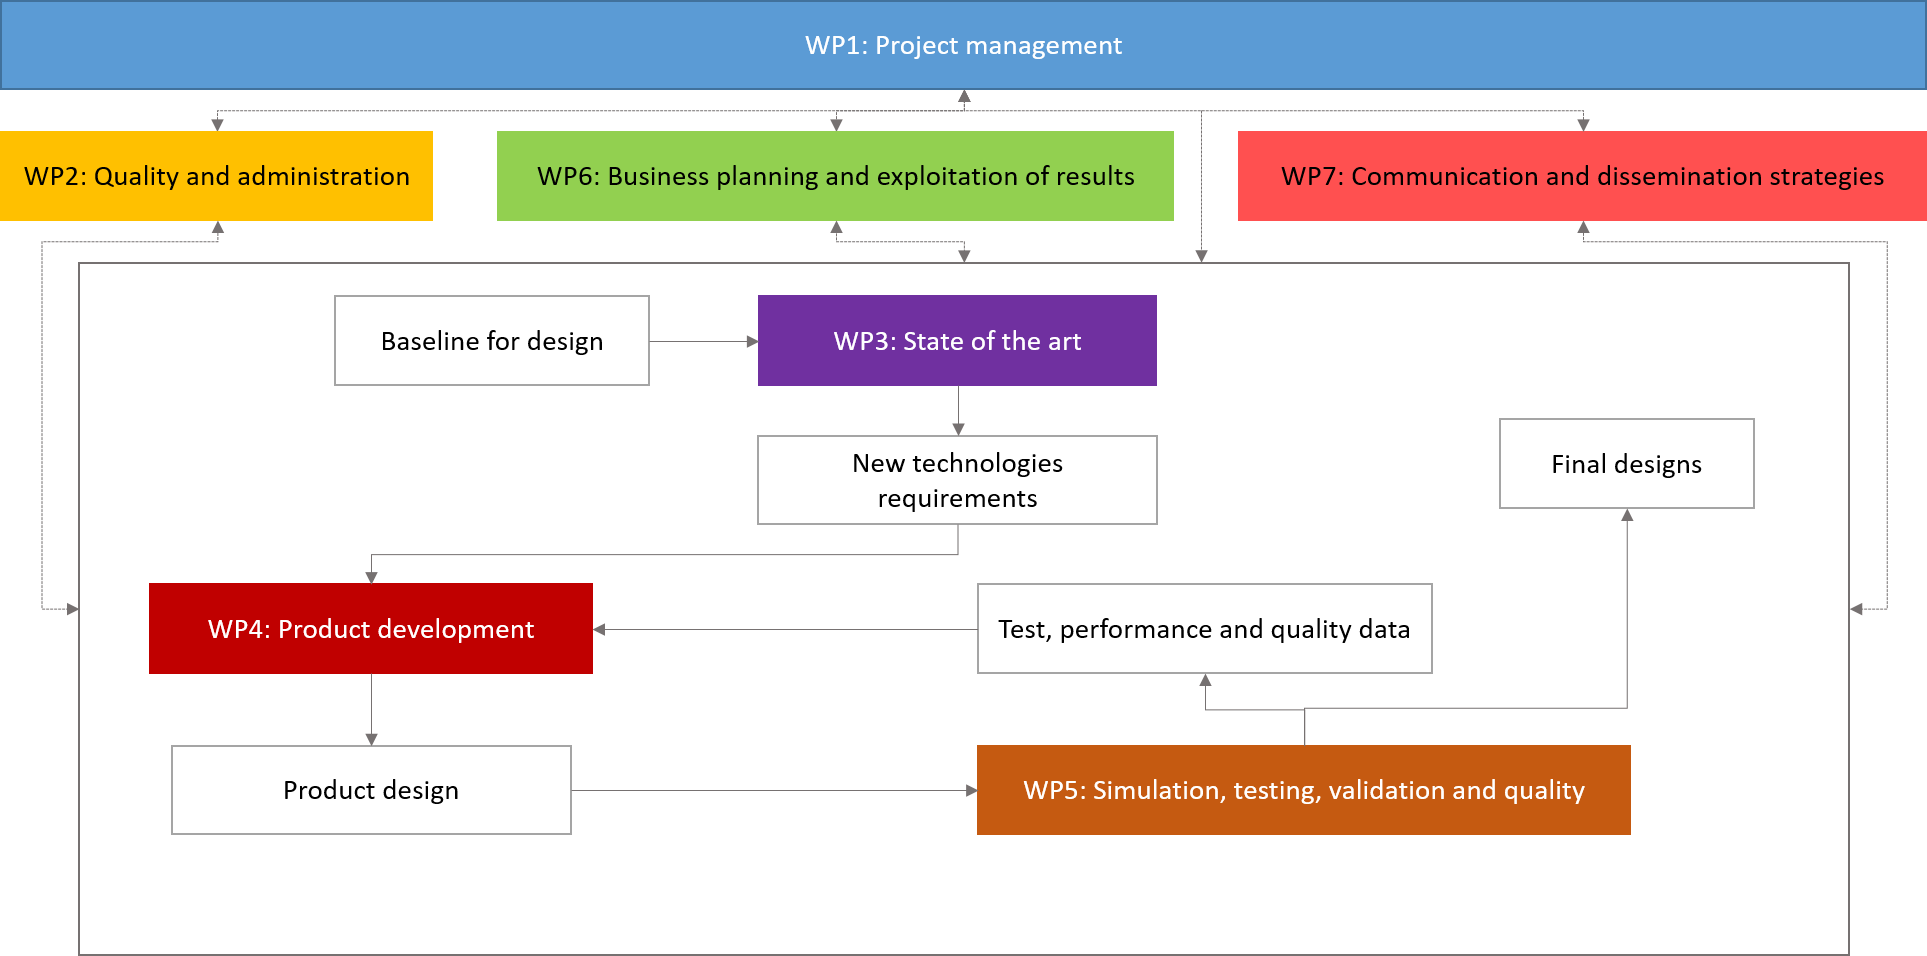
\includegraphics[width=\textwidth]{images/overallstructure.png}
\caption{DEOS-UD overall structure diagram.} 
\label{overallstructure}
\end{figure}

\subsection{Timing of the Work Plan}

Timing of the different WP: \textbf{Gantt chart. D2 Apartado 6}

\subsection{Description of Work Packages}

\begin{itemize}

\item List of WP. \textbf{D2 Apartado 2.1 Poner solo WP, no todas las activities. Extraer del D2 también Start Month i End Month}

\item Description of each WP. \textbf{Extraer información de D2 sección 2 (Número de participantes, líder, objetivos, etc.) Hay que poner las diferentes tareas dentro de cada WP y quienes participan en cada tarea. Importante: Falta calcular PM por participante. Deliverables asociados a cada WP ( también a extraer del D2).}

\end{itemize}

\begin{longtable}[H]{p{1.3cm} p{2cm} p{1.8cm} p{2cm} p{1.9cm} p{1.6cm} p{1.4cm}}
	\toprule[2pt]
	
	\textbf{Work Package No.} & \textbf{Work Package Title} & \textbf{Lead Participant No.} & \textbf{Lead Participant Short Name} & \textbf{Person Months} & \textbf{Start Month} & \textbf{End Month} \\
	
	\midrule[1.5pt] 
	\endhead
	
	 &  &  &  &  &  & \vspace{0.2cm} \\
	
	\midrule

	 &  &  &  &  &  & \vspace{0.2cm} \\
	
	\midrule
	
	 &  &  &  &  &  &  \vspace{0.2cm} \\

	\midrule

 	 &  &  &  &  &  &  \vspace{0.2cm} \\
	
	\bottomrule[2pt]
	
	\caption{List of work packages}
	\label{workpackages}
\end{longtable}


\subsection{Deliverables}

List of deliverables and milstones. \textbf{D2 sección 1.2}

KEY: Deliverable numbers in order of delivery dates. Please use the numbering convention <WP number>.<number of deliverable within that WP>.

For example, deliverable 4.2 would be the second deliverable from work package 4.

Type: Use one of the following codes:
\begin{itemize}
\item R: Document, report (excluding the periodic and final reports) 
\item DEM: Demonstrator, pilot, prototype, plan designs
\item DEC: Websites, patents filing, press i media actions, videos, etc. 
\item OTHER: Software, technical diagram, etc.
\end{itemize}

Dissemination level: Use one of the following codes:
\begin{itemize}
\item PU = Public, fully open, e.g. web
\item CO = Confidential, restricted under conditions set out in Model Grant Agreement
\item CI = Classified, information as referred to in Commission Decision 2001/844/EC.
\end{itemize}

Deliverable Date: Measured in months from the project start date (month 1)

\begin{longtable}[H]{p{1.8cm} p{2cm} p{1.3cm} p{1.8cm} p{1.3cm} p{2.1cm} p{1.8cm}}
	\toprule[2pt]
	
	\textbf{Deliverable No.} & \textbf{Deliverable Name} & \textbf{Work Package No.} & \textbf{Lead Participant Short Name} & \textbf{Type} & \textbf{Disemination Level} & \textbf{Deliverable Date} \\
	
	\midrule[1.5pt] 
	\endhead
	
	&  &  &  &  &  & \vspace{0.2cm} \\
	
	\midrule

	 &  &  &  &  &  & \vspace{0.2cm} \\
	
	\midrule
	
	 &  &  &  &  &  &  \vspace{0.2cm} \\

	\midrule

 	 &  &  &  &  &  &  \vspace{0.2cm} \\
	
	\bottomrule[2pt]
	
	\caption{List of Deliverables}
	\label{workpackages}
\end{longtable}


\subsection{Inter-relation between components}

Graphical presentation of the components showing how they inter-relate (Per chart or similar) \textbf{Algo más sencillo que el network diagram. Podría ser el network diagram.}


